\documentclass[aspectratio=169]{beamer}

% Theme settings
\usetheme{Berlin}
\usecolortheme{beaver}
\setbeamertemplate{navigation symbols}{}  % Remove navigation symbols
\setbeamertemplate{footline}[frame number]  % Show frame numbers

% Packages
\usepackage{graphicx}
\usepackage{booktabs}
\usepackage{amsmath}
\usepackage{amssymb}
\usepackage{ulem}
\usepackage{tikz}
\usepackage{multirow}
\usepackage{booktabs}
\usepackage{mathtools}
\usetikzlibrary{arrows.meta, positioning, shapes}


\newcommand{\ie}{\emph{i.e.,}\xspace}
\newcommand{\eg}{\emph{e.g.,}\xspace}
\newcommand{\st}{\emph{s.t.}\xspace}

\definecolor{darkgreen}{RGB}{0, 100, 0}
\definecolor{warn}{RGB}{100, 0, 0}
\definecolor{red}{RGB}{255, 0, 0}
\definecolor{green}{RGB}{0, 128, 0}
\definecolor{blue}{RGB}{0, 0, 255}
\newcommand{\hl}[1]{{\color{darkgreen}{#1}}}
\newcommand{\warn}[1]{{\color{warn}{#1}}}
\newcommand{\red}[1]{{\color{red}{#1}}}
\newcommand{\green}[1]{{\color{green}{#1}}}
\newcommand{\blue}[1]{{\color{blue}{#1}}}


\AtBeginSection[]{
  \begin{frame}{Outline}
    \tableofcontents[currentsection]
  \end{frame}
}


% Define MIT red color
\usepackage{xcolor}
\definecolor{mitred}{RGB}{163, 31, 52}
\newcommand{\mitred}[1]{{\color{mitred} #1}}

% Title information
\title{The Rising Lake}
\subtitle{An Intuitive Introduction to Functional Aggregate Queries}
\author{Wenchao Bai}
\institute{wbai@seu.edu.cn}
\date{\today}

\begin{document}

% Title page
\begin{frame}
    \titlepage
\end{frame}

\begin{frame}{About This Title}

\begin{block}

The unknown thing to be known appeared to me as some stretch of earth or hard marl, resisting penetration ... the sea\footnote{
We choose ``The Rising Lake'' instead of ``The Rising Sea'' as the title since FAQ spans a narrower domain than algebraic geometry.
} advances insensibly in silence, nothing seems to happen, nothing moves, the water is so far off you hardly hear it ... yet it finally surrounds the resistant substance.

\hfill --- \textit{Alexander Grothendieck}, \textit{R\'ecoltes et semailles} (1985--1987)
\end{block}

\end{frame}


\begin{frame}{About This Tutorial}
  \begin{itemize}
    \item \hl{\bf Common properties} behind optimization techniques.
    \vspace{2ex}
    \item \hl{\bf Common structure} shared by many computational problems.
    \vspace{2ex}
    \item \hl{\bf Unified language} able to express semiring problems.
    \vspace{6ex}
    \item An intuition for \hl{\bf efficient algorithms} to compute any expression in this language.
  \end{itemize}
\end{frame}

\begin{frame}{Resources}
  \begin{itemize}
    \item {\bf Course materials}: \href{https://www.ifi.uzh.ch/en/dast/teaching/EA.html}{Efficient Algorithms}\footnote{\url{https://www.ifi.uzh.ch/en/dast/teaching/EA.html}} (by Prof. Dan Olteanu, UZH)
    \vspace{2ex}
    \item {\bf Original paper}: FAQ: Questions Asked Frequently~\cite{faq} (best paper, PODS'16)
  \end{itemize}
\end{frame}

\section{Common Properties}
\begin{frame}{Example: Matrix Multiplication}
\begin{itemize}
  \item {\bf Question}: Compute $A \times B \times C$
  \item {\bf Technique}: Different parenthesizations have different cost:
  \[
    (A B) C \quad \text{vs.} \quad A (B C)
  \]
  \item \textbf{Insight:} Using \hl{\bf associativity} to choose grouping reduces computation cost.
\end{itemize}
\end{frame}

\begin{frame}{Example: Summing via MapReduce}
\begin{itemize}
  \item {\bf Question}: Sum over a large dataset distributed across nodes
  \item {\bf Technique}: Compute partial sums parallelly at different nodes, then aggregate:
  \[
     \sum_{i=1}^N x_i = \sum \text{(partial sums)}
  \]
  \item \textbf{Insight:} Using \hl{\bf commutativity} allows arbitrary order of aggregation.
\end{itemize}
\end{frame}

\begin{frame}{Example: Query Optimization}
\begin{itemize}
  \item {\bf Question}: Compute the following query:
  \[
     \sigma_{x\ge 10}(A \Join_{x} B)
  \]
  \item {\bf Technique}: Predicate pushdown:
  \[
     (\sigma_{x\ge 10}(A)) \Join_{x} (\sigma_{x\ge 10}(B))
  \]
  \item \textbf{Insight}: Using \hl{\bf distributivity} to reduce joining cost.
\end{itemize}
\vspace{1em}
\end{frame}

\begin{frame}{Takeaway: Common Properties}
\hl{\bf Associativity}, \hl{\bf commutativity}, \& \hl{\bf distributivity} are infrastructures for optimization.\looseness=-1
\end{frame}


\section{Common Structure}
\begin{frame}{Key Observation}
Computational problems commonly use
\vspace{2ex}
\begin{itemize}
  \item sequences of \hl{two binary operations}
  \vspace{1ex}
  \item applied on a \hl{finite set of values} from a given domain.
\end{itemize}
\end{frame}


\begin{frame}{Example: Shortest Distance (SD)}
\begin{center}
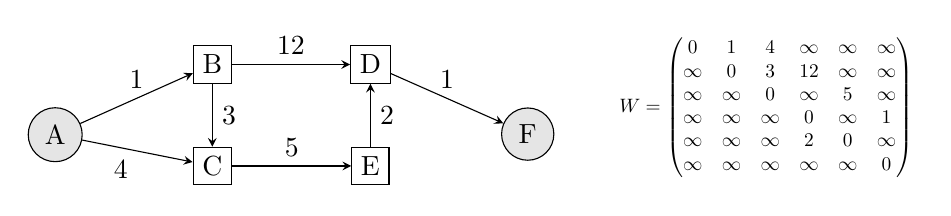
\begin{tikzpicture}[>=stealth, node distance=2cm]
\node[draw,circle,fill=gray!20] (A) {A};
\node[draw, above right=0.4cm and 1.5cm of A] (B) {B};
\node[draw, below=0.8cm of B] (C) {C};
\node[draw, right=1.5cm of B] (D) {D};
\node[draw, below=0.8cm of D] (E) {E};    
\node[draw,circle,fill=gray!20, below right=0.4cm and 1.5cm of D] (F) {F};

\draw[->] (A) -- (B) node[midway, above] {1};
\draw[->] (A) -- (C) node[midway, below left] {4};
\draw[->] (B) -- (C) node[midway, right] {3};
\draw[->] (B) -- (D) node[midway, above] {12};
\draw[->] (C) -- (E) node[midway, above] {5};
\draw[->] (E) -- (D) node[midway, right] {2};
\draw[->] (D) -- (F) node[midway, above] {1};

\node[above right=0.1cm and 0.8cm of F, anchor=west] (M) {
\scalebox{0.7}{$
W =
\begin{pmatrix}
0 & 1 & 4 & \infty & \infty & \infty\\
\infty & 0 & 3 &12 & \infty & \infty\\
\infty & \infty & 0 & \infty & 5 & \infty\\
\infty & \infty & \infty & 0 & \infty & 1\\
\infty & \infty & \infty & 2 & 0 & \infty\\
\infty & \infty & \infty & \infty & \infty & 0
\end{pmatrix}
$}
};

\end{tikzpicture}
\end{center}

\vspace{-3ex}
\begin{equation*}
\texttt{SD}(A,F)
= \min\left\{
\begin{array}{c}
  W_{A,x_1} + W_{x_1,F} \\
  \ldots \\
  W_{A,x_1} + \ldots + W_{x_{n-1},x_n} + W_{x_n,F}
\end{array}
\right\}
= \min\left\{
\begin{array}{c}
  1 + 12 + 1 \\
  4 + 5 + 2 + 1 \\
  1 + 3 + 5 + 2 + 1
\end{array}
\right\}.
\end{equation*}

\begin{itemize}
  \item \hl{\bf Binary operations}: \(\min\), \(+\)
  \item \hl{\bf Domain}: $(-\infty, \infty]$
\end{itemize}

\end{frame}

% \begin{frame}{Example [Satisfiability Problem]: Map Coloring (MC)}

% \warn{Question}: Can we color Europe's countries using only 3 colors such that no neighboring countries share the same color?

% \vspace{4ex}
% Say we use colors \red{Red}, \green{Green}, and \blue{Blue}, and for each country ({\it e.g.},~Switzerland), we use a variable ({\it e.g.},~\red{$R_{CH}$}) expressing its color. Then we can formulate as follows:

% \vspace{-2ex}
% \begin{align*}
% & (\red{R_{\text{CH}}} \lor \green{G_{\text{CH}}} \lor \blue{B_{\text{CH}}}) 
%    && \text{``CH has {\it at least} one color.''} \\
% & \land (\neg {\red{R_{\text{CH}}}} \lor \neg \green{G_{\text{CH}}}) 
%    \land (\neg \red{R_{\text{CH}}} \lor \neg \blue{B_{\text{CH}}}) 
%    \land (\neg \green{G_{\text{CH}}} \lor \neg \blue{B_{\text{CH}}}) 
%    && \text{``CH has {\it at most} one color.''} \\
% & \land (\neg \red{R_{\text{CH}}} \lor \neg \red{R_{\text{DE}}}) 
%    \land (\neg \green{G_{\text{CH}}} \lor \neg \green{G_{\text{DE}}}) 
%    \land (\neg \blue{B_{\text{CH}}} \lor \neg \blue{B_{\text{DE}}}) 
%    && \text{``CH,DE have {\it different} colors.''} \\
% & \land \dots && \dots
% \end{align*}

% \vspace{-2ex}
% \begin{itemize}
%   \item \hl{\bf Binary operations}: \(\land\), \(\lor\)
%   \item \hl{\bf Domain}: \(\{0, 1\}\)
% \end{itemize}
  
% \end{frame}

\begin{frame}{Example: Conjunctive Query (CQ)}
\begin{table}[h]
\centering
\scalebox{0.82}{%
\begin{tabular}{c c c}
% --- Table 1 ---
\begin{tabular}{l l l}
\multicolumn{3}{c}{\textbf{Orders (O for short)}}\\
\hline
customer & day & dish \\
\hline
Elise & Monday & burger \\
Elise & Friday & burger \\
Steve & Friday & hotdog \\
Joe   & Friday & hotdog \\
\hline
\end{tabular}
&
% --- Table 2 ---
\begin{tabular}{l l}
\multicolumn{2}{c}{\textbf{Dish (D for short)}}\\
\hline
dish & item \\
\hline
burger & patty \\
burger & onion \\
burger & bun \\
hotdog & sausage \\
\hline
\end{tabular}
&
% --- Table 3 ---
\begin{tabular}{l r}
\multicolumn{2}{c}{\textbf{Items (I for short)}}\\
\hline
item & price \\
\hline
patty & 6 \\
onion & 2 \\
bun   & 2 \\
sausage & 4 \\
\hline
\end{tabular}
\end{tabular}
}
\end{table}

\begin{equation*}
  \texttt{CQ}(O\bowtie D \bowtie I) = 
  \bigcup_{(v_1, v_2, v_3, v_4, v_5)} O(v_1, v_2, v_3) \cap D(v_3, v_4) \cap I(v_4, v_5)
\end{equation*}

\begin{itemize}
  \item \hl{\bf Binary operations}: \(\cup\), \(\cap\)
  \item \hl{\bf Domain}: set of tuples
\end{itemize}

\end{frame}

\begin{frame}{Common Structure Shared by These Problems}

Binary operators $\oplus$ and $\otimes$ over set $\mathbf{D}$ form a \hl{commutative semiring} ($\mathbf{D}, \oplus, \otimes, \mathbf{0}, \mathbf{1}$):\looseness=-1
\begin{itemize}
  \item $\oplus$ is associative: \hfill $a \oplus (b \oplus c) = (a \oplus b) \oplus c$
  \item $\oplus$ is commutative: \hfill $a \oplus b = b \oplus a$
  \item $\mathbf{0}$ is the additive identity: \hfill $a \oplus \mathbf{0} = a$
  \item $\otimes$ is associative: \hfill $a \otimes (b \otimes c) = (a \otimes b) \otimes c$
  \item $\otimes$ is commutative: \hfill $a \otimes b = b \otimes a$
  \item $\mathbf{1}$ is the multiplicative identity: \hfill $a \otimes \mathbf{1} = a$
  \item $\otimes$ distributes over $\oplus$: \hfill $a \otimes (b \oplus c) = (a \otimes b) \oplus (a \otimes c)$
  \item $\mathbf{0}$ is the multiplicative annihilator: \hfill $a \otimes \mathbf{0} = \mathbf{0}$
\end{itemize}
  
\vspace{2ex}
Additional condition for \hl{ring}:
\begin{itemize}
  \item each element $a$ has an additive inverse $-a$: \hfill $a \oplus (-a) = \mathbf{0}$
\end{itemize}
\end{frame}


\begin{frame}{Shortest Distance (SD) as Semiring}
  $\texttt{SD}$ forms a \hl{min-sum semiring}: $((-\infty,\infty], \min, +, \infty, 0)$:
  \begin{itemize}
    \item $\oplus = \min$ is associative: \hfill $\min(a, \min(b,c))=\min(\min(a,b), c)$
    \item $\oplus = \min$ is commutative: \hfill $\min(a,b)=\min(b,a)$
    \item $\mathbf{0} = \infty$ is the additive identity: \hfill $\min(a, \infty)=a$
    \item $\otimes = +$ is associative: \hfill $a + (b + c) = (a + b) + c$
    \item $\otimes = +$ is commutative: \hfill $a + b = b + a$
    \item $\mathbf{1} = 0$ is the multiplicative identity: \hfill $a + 0 = a$
    \item $\otimes = +$ distributes over $\oplus = \min$: \hfill $a + \min(b,c) = \min(a + b, a + c)$
    \item $\mathbf{0} = \infty$ is the multiplicative annihilator: \hfill $a + \infty = \infty$
  \end{itemize}

 \vspace{2ex}
 $\texttt{SD}$ cannot form a ring since,
 \begin{itemize}
  \item additive inverse does not exist: \hfill $\forall a\neq \infty, \nexists x\in(-\infty,\infty]$, such that $\min(a, x) = \infty$
 \end{itemize}
\end{frame}


\begin{frame}{Conjunctive Query (CQ) as Semiring}
  $\texttt{CQ}$ forms a \hl{union-intersection semiring}: $(2^\mathcal{U}, \cup, \cap, \emptyset, \mathcal{U})$:
  \begin{itemize}
    \item $\mathcal{U}$ is the cartesian product over all attributes' domains.
    \item $\oplus = \cup$ is associative: \hfill $A \cup (B \cup C) = (A \cup B) \cup C$
    \item $\oplus = \cup$ is commutative: \hfill $A \cup B = B \cup A$
    \item $\mathbf{0} = \emptyset$ is the additive identity: \hfill $A \cup \emptyset = A$
    \item $\otimes = \cap$ is associative: \hfill $A \cap (B \cap C) = (A \cap B) \cap C$
    \item $\otimes = \cap$ is commutative: \hfill $A \cap B = B \cap A$
    \item $\mathbf{1} = \mathcal{U}$ is the multiplicative identity: \hfill $A \cap \mathcal{U} = A$
    \item $\otimes = \cap$ distributes over $\oplus = \cup$: \hfill $A \cap (B \cup C) = (A \cap B) \cup (A \cap C)$
    \item $\mathbf{0} = \emptyset$ is the multiplicative annihilator: \hfill $A \cap \emptyset = \emptyset$
  \end{itemize}

  \vspace{2ex}
  $\texttt{CQ}$ cannot form a ring since,
  \begin{itemize}
    \item additive inverse does not exist: \hfill $\forall A\neq \emptyset, \nexists X\in 2^\mathcal{U}$, such that $A \cup X = \emptyset$
  \end{itemize}
\end{frame}

\begin{frame}{Sample Problems and Their Semirings%
\footnote{See topic 2 (Commutative Semirings) for more detail: \url{https://www.ifi.uzh.ch/en/dast/teaching/EA.html}}}

\scriptsize
\begin{table}
\centering
\renewcommand{\arraystretch}{1.5}
\begin{tabular}{l l l c c c c c}
\hline
\textbf{Category} & \textbf{Problem} & \textbf{Type} & \textbf{Domain} & $\oplus$ & $\otimes$ & $\mathbf{0}$ & $\mathbf{1}$ \\
\hline

\multirow{4}{*}{Path Queries}
  & Shortest Distance & Min–Sum
  & $(-\infty,\infty]$ & $\min$ & $+$ & $\infty$ & $0$ \\

  & Connectivity & Boolean
  & $\{\texttt{F},\texttt{T}\}$ & $\lor$ & $\land$ & $\texttt{F}$ & $\texttt{T}$ \\

  & Largest Capacity & Max–Min
  & $[-\infty,\infty]$ & $\max$ & $\min$ & $-\infty$ & $\infty$ \\

  & Maximum Reliability & Max–Product
  & $[0,1]$ & $\max$ & $\times$ & $0$ & $1$ \\
\hline

Satisfiability
  & Map Coloring & Boolean
  & $\{\texttt{F},\texttt{T}\}$ & $\lor$ & $\land$ & $\texttt{F}$ & $\texttt{T}$ \\
\hline

\multirow{2}{*}{Database Queries}
  & Conjunctive Queries & Union–Intersection
  & $2^\mathcal{U}$ & $\cup$ & $\cap$ & $\emptyset$ & $\mathcal{U}$ \\

  & Factorised Agg-Joins & Sum–Product
  & $\mathbb{Z}$ & $+$ & $\times$ & $0$ & $1$ \\
\hline
\ldots & \ldots & \ldots & \ldots & \ldots & \ldots & \ldots & \ldots \\
\hline
\end{tabular}
\end{table}

\end{frame}


\begin{frame}{Takeaway: The Power of Semirings}
\hl{\bf Why are Semirings Relevant in Computer Science?}
\begin{itemize}
  \item They enable generic problem solving
  \begin{itemize}
    \item by changing the semiring, the algorithm remains the same
  \end{itemize}
  \item They reduce computational complexity
  \begin{itemize}
    \item thanks to the \underline{\bf distributivity} law
  \end{itemize}
  \item Permutability is an important property behind optimization techniques.
  \begin{itemize}
    \item thanks to the \underline{\bf associativity} and \underline{\bf commutativity} laws
  \end{itemize}
\end{itemize}

\vspace{2ex}
\hl{\bf Different semirings give different semantics of}
\begin{itemize}
  \item the same problem
  \item the same algorithm
  \item the same complexity
  \item the same implementation
\end{itemize}
\end{frame}

\section{Unified Language}

\begin{frame}{Functional Aggregate Query: The Input (1/2)}

\begin{figure}
\centering
\includegraphics[width=0.7\textwidth]{figs/faq_demo.pdf}
\end{figure}

\begin{itemize}
  \item Variables: $\mathcal{V}=\{X_1,\ldots,X_n\}$
  \begin{itemize}
    \item $F\subseteq \mathcal{V}$: free variables (input variables)\footnote{{\it w.l.o.g.},~$F=\mathbf{X}_{[f]}=\{X_1,\ldots,X_f\}$, {\it i.e.},~the first $f$ variables.}, {\it e.g.},~$X_1$ is a free variable of $\varphi(X_1)$. 
    \item $\mathcal{V}\setminus F$: bound variables, {\it e.g.},~$\{X_2,X_3,X_4\}$ are bound variables of $\varphi(X_1)$.
    \item {\it E.g.},~in the query $\texttt{SD}(A,B)$ ``the shortest dist. between $A$ and $B$'', $F=\{A,B\}$.
  \end{itemize}
\end{itemize}
 
\end{frame}


\begin{frame}{Functional Aggregate Query: The Input (2/2)}

\begin{figure}
\centering
\includegraphics[width=0.7\textwidth]{figs/faq_demo.pdf}
\end{figure}

\begin{itemize}
  \item Variables: $\mathcal{V}=\{X_1,\ldots,X_n\}$
  \vspace{1ex}
  \item Multi-Hypergraph: $\mathcal{H}=(\mathcal{V}, \mathcal{E})$
  \begin{itemize}
    \item $\mathcal{V}$: set of vertices (variables) 
    \item $\mathcal{E}\subseteq 2^{[n]}$: $\forall S\in\mathcal{E}$, we have a factor $\psi_S$. All factors have the same range $\mathbf{D}$.
    
    \begin{equation*}
    \psi_S: \prod_{i\in S} \text{Dom}(X_i) \to \mathbf{D}
    \end{equation*}
  \end{itemize}
\end{itemize}
 
\end{frame}


\begin{frame}{Functional Aggregate Query: The Output}

\begin{figure}
\centering
\includegraphics[width=0.7\textwidth]{figs/faq_demo.pdf}
\end{figure}

\begin{itemize}
  \item Compute the function $\varphi: \prod_{i\in F} \text{Dom}(X_i) \to \mathbf{D}$.
  \item $\varphi$ is defined by the \hl{\bf FAQ-Expression}:
  \begin{equation*}
    \varphi(\mathbf{x}_{[F]}) = \blue{\bigoplus^{(f+1)}_{x_{f+1}\in \texttt{Dom}(X_{f+1})}} \ldots \green{\bigoplus^{(n)}_{x_{n}\in \texttt{Dom}(X_{n})}}\bigotimes_{S\in \mathcal{E}} \psi_S(\mathbf{x}_S)
  \end{equation*}
  \item For each $\oplus^{(i)}$, either $(\mathbf{D}, \oplus^{(i)}, \otimes, \mathbf{0}, \mathbf{1})$ is a commutative semiring, or $\oplus^{(i)}=\otimes$.
\end{itemize}

\end{frame}


\begin{frame}{Path Query as FAQ (1/5)}
 \begin{center}
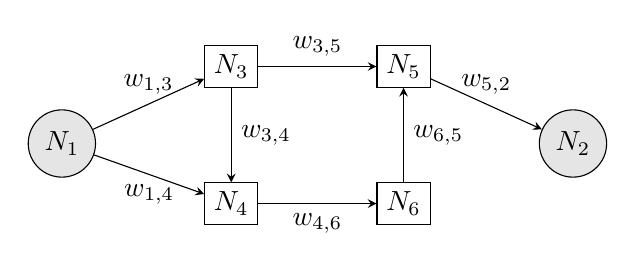
\begin{tikzpicture}[>=stealth, node distance=2cm]
\node[draw,circle,fill=gray!20] (X1) {$N_1$};
\node[draw, above right=0.4cm and 1.5cm of X1] (X3) {$N_3$};
\node[draw, below=1.2cm of X3] (X4) {$N_4$};
\node[draw, right=1.5cm of X3] (X5) {$N_5$};
\node[draw, below=1.2cm of X5] (X6) {$N_6$};    
\node[draw,circle,fill=gray!20, below right=0.4cm and 1.5cm of X5] (X2) {$N_2$};
\draw[->] (X1) -- (X3) node[midway, above] {$w_{1,3}$};
\draw[->] (X1) -- (X4) node[midway, below] {$w_{1,4}$};
\draw[->] (X3) -- (X4) node[midway, right] {$w_{3,4}$};
\draw[->] (X3) -- (X5) node[midway, above] {$w_{3,5}$};
\draw[->] (X4) -- (X6) node[midway, below] {$w_{4,6}$};
\draw[->] (X6) -- (X5) node[midway, right] {$w_{6,5}$};
\draw[->] (X5) -- (X2) node[midway, above] {$w_{5,2}$};

\end{tikzpicture}
\end{center} 


\begin{itemize}
  \item Variables $\mathcal{V}$: $\{X_1,\ldots,X_6\}$, where $\forall X_i\in\mathcal{V},~\texttt{Dom}(X_i)=V(G)=\{N_1,\ldots,N_6\}$.
  \item Free variables $F$: $\{X_1,X_2\}$ are assigned as the source and target vertices.
  \item Hyperedges $\mathcal{E}$: vertex pair $E(G)=V(G)^2$.
  \item Factors $\psi_S$: function $\mathcal{E}\rightarrow \mathbf{D}$, where $S\in \mathcal{E}$.
\end{itemize}

\end{frame}


\begin{frame}{Path Query as FAQ (2/5)}

\vspace{-3ex}
\begin{align*}
  \varphi(\mathbf{x}_{[2]}) &= \bigoplus_{x_{3},x_{4},x_{5},x_{6}\in V(G)} \bigotimes_{S\in \mathcal{E}} \psi_S(\mathbf{x}_S)\\
  &=\psi(N_1,N_2) \oplus \left(\bigoplus_{x_3\in V(G)}\psi(N_1,x_3)\otimes\psi(x_3,N_2)\right) && \text{// 1 and 2 hops} \\
  &=\ldots &&\text{// 3 and 4 hops} \\
  &=\oplus \left(\bigoplus_{x_3,\ldots,x_6\in V(G)}\psi(N_1,x_3)\otimes\psi(x_3,x_4)\otimes\ldots\otimes\psi(x_6,N_2)\right) && \text{// 5 hops} \\
\end{align*}

\vspace{-2ex}
\begin{itemize}
  \item \hl{\bf Shortest distance}: $\oplus=\min$, $\otimes=+$, $\psi$ returns edge weights, $\mathbf{D}=\mathbb{R}\cup\{\infty\}$
\end{itemize}

\end{frame}


\begin{frame}{Path Query as FAQ (3/5)}

\vspace{-3ex}
\begin{align*}
  \varphi(\mathbf{x}_{[2]}) &= \bigoplus_{x_{3},x_{4},x_{5},x_{6}\in V(G)} \bigotimes_{S\in \mathcal{E}} \psi_S(\mathbf{x}_S)\\
  &=\psi(N_1,N_2) \oplus \left(\bigoplus_{x_3\in V(G)}\psi(N_1,x_3)\otimes\psi(x_3,N_2)\right) && \text{// 1 and 2 hops} \\
  &=\ldots &&\text{// 3 and 4 hops} \\
  &=\oplus \left(\bigoplus_{x_3,\ldots,x_6\in V(G)}\psi(N_1,x_3)\otimes\psi(x_3,x_4)\otimes\ldots\otimes\psi(x_6,N_2)\right) && \text{// 5 hops} \\
\end{align*}

\vspace{-2ex}
\begin{itemize}
  \item \hl{\bf Largest capacity}: $\oplus=\max$, $\otimes=\min$, $\psi$ returns edge weights, $\mathbf{D}=\mathbb{R}\cup\{-\infty,\infty\}$\looseness=-1
\end{itemize}

\end{frame}

\begin{frame}{Path Query as FAQ (4/5)}

\vspace{-3ex}
\begin{align*}
  \varphi(\mathbf{x}_{[2]}) &= \bigoplus_{x_{3},x_{4},x_{5},x_{6}\in V(G)} \bigotimes_{S\in \mathcal{E}} \psi_S(\mathbf{x}_S)\\
  &=\psi(N_1,N_2) \oplus \left(\bigoplus_{x_3\in V(G)}\psi(N_1,x_3)\otimes\psi(x_3,N_2)\right) && \text{// 1 and 2 hops} \\
  &=\ldots &&\text{// 3 and 4 hops} \\
  &=\oplus \left(\bigoplus_{x_3,\ldots,x_6\in V(G)}\psi(N_1,x_3)\otimes\psi(x_3,x_4)\otimes\ldots\otimes\psi(x_6,N_2)\right) && \text{// 5 hops} \\
\end{align*}

\vspace{-2ex}
\begin{itemize}
  \item \hl{\bf Connectivity}: $\oplus=\lor$, $\otimes=\land$, $\psi$ returns edge existance, $\mathbf{D}=\{\texttt{F}, \texttt{T}\}$
\end{itemize}

\end{frame}


\begin{frame}{Path Query as FAQ (5/5)}

\vspace{-3ex}
\begin{align*}
  \varphi(\mathbf{x}_{[2]}) &= \bigoplus_{x_{3},x_{4},x_{5},x_{6}\in V(G)} \bigotimes_{S\in \mathcal{E}} \psi_S(\mathbf{x}_S)\\
  &=\psi(N_1,N_2) \oplus \left(\bigoplus_{x_3\in V(G)}\psi(N_1,x_3)\otimes\psi(x_3,N_2)\right) && \text{// 1 and 2 hops} \\
  &=\ldots &&\text{// 3 and 4 hops} \\
  &=\oplus \left(\bigoplus_{x_3,\ldots,x_6\in V(G)}\psi(N_1,x_3)\otimes\psi(x_3,x_4)\otimes\ldots\otimes\psi(x_6,N_2)\right) && \text{// 5 hops} \\
\end{align*}

\vspace{-2ex}
\begin{itemize}
  \item \hl{\bf Shortest path}: $\oplus=\cup$, $\otimes=\warn{\texttt{\bf concat}}$, $\psi$ returns edge itself or $\emptyset$, $\mathbf{D}=E(G)\cup\{\emptyset\}$
\end{itemize}

\end{frame}


\begin{frame}{DB Query as FAQ (1/3)}

\begin{figure}
\centering
\includegraphics[width=0.6\textwidth]{figs/cq_demo.png}
\end{figure}
  
\begin{itemize}
  \item \texttt{Q1}: \texttt{SELECT * FROM Orders NATURAL JOIN Dish NATURAL JOIN Items;}
  \item {\bf FAQ} over \hl{union-intersection} semiring, where $\psi$ maps tuple to $\{\emptyset, \{\text{tuple}\}\}$:
  \begin{equation*}
    \varphi() = \bigcup_{x_1,x_2,x_3,x_4,x_5} \psi_{1,2,3}(x_1,x_2,x_3) \cap \psi_{3,4}(x_3,x_4) \cap \psi_{4,5}(x_4,x_5)
  \end{equation*}
\end{itemize}
\end{frame}



\begin{frame}{DB Query as FAQ (2/3)}

\begin{figure}
\centering
\includegraphics[width=0.6\textwidth]{figs/cq_demo.png}
\end{figure}
  
\begin{itemize}
  \item \texttt{Q2}: \texttt{SELECT customer,COUNT(*) from Q1 GROUP BY customer;}
  \item {\bf FAQ} over \hl{sum-product} semiring, where $\psi$ maps tuple to $\{0,1\}$:
  \begin{equation*}
    \varphi(x_1) = \sum_{x_2,x_3,x_4,x_5} \psi_{1,2,3}(x_1,x_2,x_3) \cdot \psi_{3,4}(x_3,x_4) \cdot \psi_{4,5}(x_4,x_5)
  \end{equation*}
\end{itemize}
\end{frame}


\begin{frame}{DB Query as FAQ (3/3)}

\begin{figure}
\centering
\includegraphics[width=0.6\textwidth]{figs/cq_demo.png}
\end{figure}
  
\begin{itemize}
  \item \texttt{Q3}: \texttt{SELECT customer,day,SUM(price) from Q1 GROUP BY customer,day;}
  \item {\bf FAQ} over \hl{sum-product} semiring, where $\psi_{4,5}$ maps $(x_4,x_5)$ to $x_5$; others are the same as \texttt{Q2}:
  \begin{equation*}
    \varphi(x_1,x_2) = \sum_{x_3,x_4,x_5} \psi_{1,2,3}(x_1,x_2,x_3) \cdot \psi_{3,4}(x_3,x_4) \cdot \psi_{4,5}(x_4,x_5)
  \end{equation*}
\end{itemize}
\end{frame}


\begin{frame}{Takeaway: A Unified Language}
  \begin{itemize}
    \item FAQ is a \hl{unified language} to express many problems in computer science.
    \item See appendix for more problems expressible in FAQ over different semirings.
  \end{itemize}
\end{frame}


\section{Efficient algorithms}

\begin{frame}{The Nature of FAQ}
  \begin{itemize}
    \item A collection of \hl{factors}.
    \item A \hl{hypergraph} to guide the factor assembling.
  \end{itemize}
\end{frame}


\begin{frame}{Hypergraphs: The Good and The Bad}
Consider the following two FAQs. $\varphi_2$ is the same as $\varphi_2$ in the case when $X_4=X_1$.

\vspace{2ex}
\begin{itemize}
  \item {\bf Acyclic FAQ}: $\varphi_1=\bigoplus{\mathbf{x}_{[4]}} \psi_{1,2}(x_1,x_2) \otimes \psi_{2,3}(x_2,x_3) \otimes \psi_{3,4}(x_3,x_4)$
  \vspace{1ex}
  \item {\bf Cyclic FAQ}: $\varphi_2=\bigoplus{\mathbf{x}_{[3]}} \psi_{1,2}(x_1,x_2) \otimes \psi_{2,3}(x_2,x_3) \otimes \psi_{3,1}(x_1,x_3)$
\end{itemize}


\vspace{2ex}
\begin{columns}
\begin{column}{0.2\textwidth}
\centering
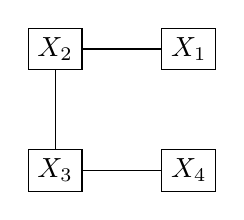
\begin{tikzpicture}
\node[draw] (X2) {$X_2$};
\node[draw, right=1cm of X2] (X1) {$X_1$};
\node[draw, below=1cm of X2] (X3) {$X_3$};
\node[draw, right=1cm of X3] (X4) {$X_4$};
\draw (X1) -- (X2);
\draw (X2) -- (X3);
\draw (X3) -- (X4);
\end{tikzpicture}

\vspace{1ex}
\small Hypergraph of $\varphi_1$.
\end{column}

\begin{column}{0.2\textwidth}
\centering
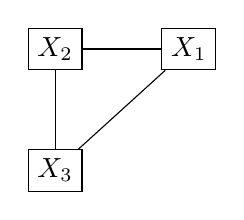
\begin{tikzpicture}
\node[draw] (X2) {$X_2$};
\node[draw, right=1cm of X2] (X1) {$X_1$};
\node[draw, below=1cm of X2] (X3) {$X_3$};
\draw (X1) -- (X2) node[midway, above] {};
\draw (X2) -- (X3) node[midway, below] {};
\draw (X3) -- (X1) node[midway, right] {};
\end{tikzpicture}

\vspace{1ex}
\small Hypergraph of $\varphi_2$.
\end{column}
\end{columns}

\end{frame}


\begin{frame}{Example: The Acyclic FAQ over Boolean Semiring (1/2)}
\begin{center}
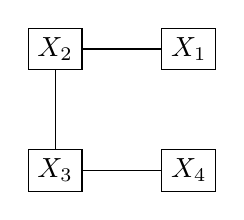
\begin{tikzpicture}
\node[draw] (X2) {$X_2$};
\node[draw, right=1cm of X2] (X1) {$X_1$};
\node[draw, below=1cm of X2] (X3) {$X_3$};
\node[draw, right=1cm of X3] (X4) {$X_4$};
\draw (X1) -- (X2);
\draw (X2) -- (X3);
\draw (X3) -- (X4);
\end{tikzpicture}
\end{center}

Consider the instance of $\varphi_1$ over the Boolean semiring:
\begin{equation*}
  \varphi=\bigvee_{\mathbf{x}_{[4]}\in\prod_{i\in[4]}\texttt{Dom}(X_i)} \psi_{1,2}(x_1,x_2) \land \psi_{2,3}(x_2,x_3) \land \psi_{3,4}(x_3,x_4)
\end{equation*}

\vspace{2ex}
$\varphi$ asks whether there's a tuple $(x_1,\ldots,x_4)$ such that all factors $\psi_{i,j}(x_i,x_j)=\texttt{True}$.

\end{frame}

\begin{frame}{Example: The Acyclic FAQ over Boolean Semiring (2/2)}
\begin{columns}
\begin{column}{0.2\textwidth}
\centering
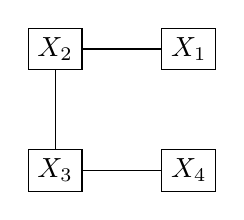
\begin{tikzpicture}
\node[draw] (X2) {$X_2$};
\node[draw, right=1cm of X2] (X1) {$X_1$};
\node[draw, below=1cm of X2] (X3) {$X_3$};
\node[draw, right=1cm of X3] (X4) {$X_4$};
\draw (X1) -- (X2);
\draw (X2) -- (X3);
\draw (X3) -- (X4);
\end{tikzpicture}
\end{column}
\begin{column}{0.2\textwidth}
\centering
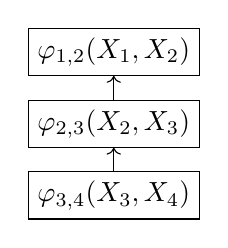
\begin{tikzpicture}
\node[draw] (X1) {$\varphi_{1,2}(X_1,X_2)$};
\node[draw, below=0.3cm of X1] (X2) {$\varphi_{2,3}(X_2,X_3)$};
\node[draw, below=0.3cm of X2] (X3) {$\varphi_{3,4}(X_3,X_4)$};
\draw[->] (X2) -- (X1);
\draw[->] (X3) -- (X2);
\end{tikzpicture}
\end{column}
\end{columns}

\vspace{0.5ex}
\begin{equation*}
  \varphi=\bigvee_{\mathbf{x}_{[4]}\in\prod_{i\in[4]}\texttt{Dom}(X_i)} \psi_{1,2}(x_1,x_2) \land \psi_{2,3}(x_2,x_3) \land \psi_{3,4}(x_3,x_4)
\end{equation*}

\vspace{0.5ex}
\begin{itemize}
  \item[@$\varphi_{3,4}$] Send up $x_4$-values: $V_{(3,4)\rightarrow (2,3)}(x_4) = \bigvee_{x_3}\psi_{3,4}(x_3,x_4)$
  \item[@$\varphi_{2,3}$] Send up $x_2$-values: $V_{(2,3)\rightarrow (1,2)}(x_2) = \bigvee_{x_3}\psi_{2,3}(x_2,x_3) \land V_{(3,4)\rightarrow (2,3)}(x_3)$
  \item[@$\varphi_{1,2}$] Sum up: $\varphi()=\bigvee_{x_1}\psi_{1,2}(x_1,x_2) \land V_{(2,3)\rightarrow (1,2)}(x_2)$ 
\end{itemize}


\end{frame}


\begin{frame}{The Power of Acyclicity}
\hl{All computation steps are local and their cost upper bounded by the factor sizes}
\vspace{1ex}
\begin{itemize}
  \item Typical assumption: $|\psi_{i,j}|\le N$ for some value $N$.
  \item We pass along at most $N$ values between factors.
  \item Local computation is just filtering local values with incoming values.
  \item \hl{Overall: linear computation time - This is the best in the worst case.}
\end{itemize}

\vspace{2ex}
Evaluation strategy know for decades under different names:
\begin{itemize}
  \item Message passing~\cite{pearl2022fusion} (in AI literatures)
  \item Semi-Join reduction~\cite{yannakakis1981algorithms} (in DB literatures)
\end{itemize}
\end{frame}

\begin{frame}{The Bad Case: Cyclic FAQs (1/2)}
 \begin{columns}
\begin{column}{0.2\textwidth}
\centering
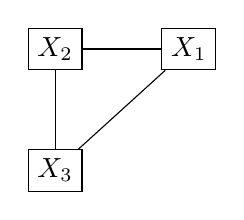
\begin{tikzpicture}
\node[draw] (X2) {$X_2$};
\node[draw, right=1cm of X2] (X1) {$X_1$};
\node[draw, below=1cm of X2] (X3) {$X_3$};
\draw (X1) -- (X2);
\draw (X2) -- (X3);
\draw (X3) -- (X1);
\end{tikzpicture}
\end{column}
\begin{column}{0.2\textwidth}
\centering
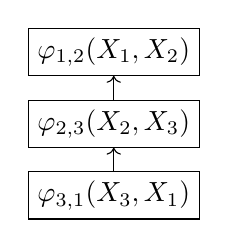
\begin{tikzpicture}
\node[draw] (X1) {$\varphi_{1,2}(X_1,X_2)$};
\node[draw, below=0.3cm of X1] (X2) {$\varphi_{2,3}(X_2,X_3)$};
\node[draw, below=0.3cm of X2] (X3) {$\varphi_{3,1}(X_3,X_1)$};
\draw[->] (X2) -- (X1);
\draw[->] (X3) -- (X2);
\end{tikzpicture}
\end{column}
\end{columns}

\vspace{0.5ex}
\begin{equation*}
  \varphi'=\bigvee_{\mathbf{x}_{[3]}\in\prod_{i\in[3]}\texttt{Dom}(X_i)} \psi_{1,2}(x_1,x_2) \land \psi_{2,3}(x_2,x_3) \land \psi_{3,1}(x_3,x_1)
\end{equation*}

\vspace{0.5ex}
\begin{itemize}
  \item[@$\varphi_{3,1}$] Send up $(x_1,x_3)$-values: $V_{(3,1)\rightarrow (2,3)}(x_1,x_3) = \psi_{3,1}(x_3,x_1)$
  \item[@$\varphi_{2,3}$] Send up $(x_1,x_2)$-values: \warn{\bf $V_{(2,3)\rightarrow (1,2)}(x_1,x_2) = \bigvee_{x_3}\psi_{2,3}(x_2,x_3) \land V_{(3,1)\rightarrow (2,3)}(x_1,x_3)$}
  \item[@$\varphi_{1,2}$] Sum up: $\varphi'()=\bigvee_{x_1,x_2}\psi_{1,2}(x_1,x_2) \land V_{(2,3)\rightarrow (1,2)}(x_1, x_2)$ 
\end{itemize} 
\end{frame}


\begin{frame}{The Bad Case: Cyclic FAQs (2/2)}
 \begin{columns}
\begin{column}{0.2\textwidth}
\centering
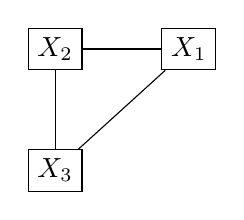
\begin{tikzpicture}
\node[draw] (X2) {$X_2$};
\node[draw, right=1cm of X2] (X1) {$X_1$};
\node[draw, below=1cm of X2] (X3) {$X_3$};
\draw (X1) -- (X2);
\draw (X2) -- (X3);
\draw (X3) -- (X1);
\end{tikzpicture}
\end{column}
\begin{column}{0.2\textwidth}
\centering
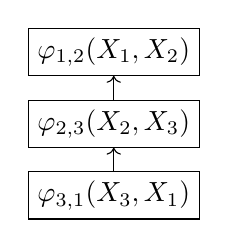
\begin{tikzpicture}
\node[draw] (X1) {$\varphi_{1,2}(X_1,X_2)$};
\node[draw, below=0.3cm of X1] (X2) {$\varphi_{2,3}(X_2,X_3)$};
\node[draw, below=0.3cm of X2] (X3) {$\varphi_{3,1}(X_3,X_1)$};
\draw[->] (X2) -- (X1);
\draw[->] (X3) -- (X2);
\end{tikzpicture}
\end{column}
\end{columns}

\vspace{0.5ex}
\begin{equation*}
  \varphi'=\bigvee_{\mathbf{x}_{[3]}\in\prod_{i\in[3]}\texttt{Dom}(X_i)} \psi_{1,2}(x_1,x_2) \land \psi_{2,3}(x_2,x_3) \land \psi_{3,1}(x_3,x_1)
\end{equation*}

\vspace{2ex}
$V_{(2,3)\rightarrow (1,2)} = \bigvee_{x_3}\psi_{2,3}(x_2,x_3) \land V_{(3,1)\rightarrow (2,3)}(x_1,x_3)$ introduces \warn{$O(N^2)$} cost.
\vspace{1ex}
\begin{itemize}
  \item It's a join instead of a semi-join.
\end{itemize}
\end{frame}

\begin{frame}{A Roadmap for Further Study}

\begin{enumerate}
  \item Can we distinguish syntatically the acyclic from the cyclic hypergraphs?
  \begin{itemize}
    \item $\alpha$-acyclic, $\beta$-acyclic, free-connex, {\it etc.}
  \end{itemize}
  \vspace{1ex}
  \item How to transform cyclic hypergraphs to acyclic ones?
  \begin{itemize}
    \item Hypertree decomposition.
  \end{itemize}
  \vspace{1ex}
  \item How to measure the goodness of such transformations?
  \begin{itemize}
    \item Width measures: hypertree width, fractional hypertree width, {\it etc.}
  \end{itemize}
  \vspace{1ex}
  \item How to design efficient algorithms for FAQs over (commutative) semirings?
  \begin{itemize}
    \item InsideOut algorithm~\cite{faq}.
  \end{itemize}
\end{enumerate}
  
\end{frame}


\section*{Appendix}
\label{sec:appendix}
\begin{frame}{Problems Expressible in FAQ over Boolean Semiring}

  {\bf $(\{\texttt{F}, \texttt{T}\}, \lor, \land, \texttt{F}, \texttt{T})$}

  \begin{itemize}
    \item Constraint satisfaction problems (CSP) \hfill FAQ~\cite{faq}
    \item Boolean conjunctive query evaluation (BCQ) \hfill FAQ~\cite{faq}
    \item Conjunctive query evaluation (CQ)\footnote{it's also expressible using the set semiring.} \hfill FAQ~\cite{faq}
    \item Join evaluation \hfill FAQ~\cite{faq}
    \item Satisfiability (SAT) \hfill FAQ~\cite{faq}
    \item $k$-colorability \hfill FAQ~\cite{faq}
    \item List recovery problem (coding theory) \hfill FAQ~\cite{faq}
  \end{itemize}

\end{frame}

\begin{frame}{Problems Expressible in FAQ over Set Sum-Product Semiring}

  {\bf $(2^{\mathcal{U}}, \cup, \cap, \emptyset, \mathcal{U})$}

  \begin{itemize}
    \item Conjunctive query evaluation (CQ)\footnote{It's also expressible using the Boolean semiring.} \hfill FAQ~\cite{faq}
    \item Join evaluation \hfill FAQ~\cite{faq}
  \end{itemize}
\end{frame}

\begin{frame}{Problems Expressible in FAQ over Natural Sum-Product Semiring}

  {\bf $(\mathbb{N}, +, \times, 0, 1)$}
  
  \begin{itemize}
    \item Complex network analysis \hfill FAQ~\cite{faq}
    \item Count constraint satisfaction problems (\#CSP) \hfill FAQ~\cite{faq}
    \item Count satisfiability (\#SAT) \hfill FAQ~\cite{faq}
  \end{itemize}

\end{frame}

\begin{frame}{Problems Expressible in FAQ over Real Sum-Product Semiring}

  {\bf $(\mathbb{R}, +, \times, 0, 1)$}


  \begin{itemize}
    \item Permanent \hfill FAQ~\cite{faq}
    \item Discrete Fourier transform \hfill FAQ~\cite{faq},AjiMcEl~\cite{AjiMcEl}
    \item Hadamard transform \hfill AjiMcEl~\cite{AjiMcEl}
    \item Inference in probabilistic graphical models \hfill FAQ~\cite{faq}
    \item Probability propagation in AI \hfill AjiMcEl~\cite{AjiMcEl}
    \item Matrix chain multiplication \hfill FAQ~\cite{faq},AjiMcEl~\cite{AjiMcEl}
    \item Graph homomorphism \hfill FAQ~\cite{faq}
    \item BCJR decoding (Bahl, Cocke, Jelinek, Raviv) \hfill AjiMcEl~\cite{AjiMcEl}
    \item Holant problem \hfill FAQ~\cite{faq}
  \end{itemize}

\end{frame}

\begin{frame}{Problems Expressible in FAQ over Max-Product Semiring}

  {\bf $([0,\infty), \max, \times, 0, 1)$}

  \begin{itemize}
    \item MAP queries in probabilistic graphical models \hfill FAQ~\cite{faq}
    \item Quantified conjunctive query evaluation (QCQ)\footnote{It's also expressible using the max-product, min-product semirings.} \hfill FAQ~\cite{faq}
  \end{itemize}

\end{frame}

\begin{frame}{Problems Expressible in FAQ over Min-Sum Semiring}

  {\bf $((-\infty,\infty], \min, +, \infty, 0)$}

  \begin{itemize}
    \item Gallager-Tanner-Wiberg decoding \hfill AjiMcEl~\cite{AjiMcEl}
    \item Viterbi decoding \hfill AjiMcEl~\cite{AjiMcEl}
    \item Trellis path problem \hfill AjiMcEl~\cite{AjiMcEl}
    \item Graph optimization \hfill KohlWils~\cite{KohlWils}
    \item Queuing systems \hfill KohlWils~\cite{KohlWils}
    \item Discrete event systems \hfill KohlWils~\cite{KohlWils}
    \item Optimization for weighted CSPs \hfill KohlWils~\cite{KohlWils}
  \end{itemize}

\end{frame}

\begin{frame}{Problems Expressible in FAQ over Two Semiring}

  {\bf $([0,\infty), \max, \times, 0, 1), ((0, \infty], \min, \times, \infty, 1)$}
  \begin{itemize}
    \item Quantified conjunctive query evaluation (QCQ)\footnote{It's also expressible using the max-product semiring} \hfill FAQ~\cite{faq}
  \end{itemize}

  \vspace{2ex}
  {\bf $(\mathbb{N}, \max, \times, 0, 1), (\mathbb{N}, +, \times, 0, 1)$}

  \begin{itemize}
    \item Count conjunctive query evaluation (\#CQ) \hfill FAQ~\cite{faq}
    \item Count quantified conjunctive query evaluation (\#QCQ) \hfill FAQ~\cite{faq}
  \end{itemize}

\end{frame}



\section*{Reference}
% Reference from a .bib file
\begin{frame}[allowframebreaks]{References}
    % \nocite{*}
    \renewcommand{\refname}{} 
    \bibliographystyle{plain} 
    \bibliography{references}
\end{frame}


\end{document}